\documentclass[12pt]{article}

\usepackage{graphicx}
\usepackage[margin=1in]{geometry}
\usepackage{setspace}
\onehalfspacing


\title{Early Status Report}
\author{
	Dustin Allen
	\and
	Daniel Armas
	\and
	Rithik Dhakshnamoorthy
	\and
	Jacob Plotz
	\and
	Luke Samuel Sandoval
	\and
	Jereme Saunders
}
\date{\today}

\begin{document}

\maketitle

\section{Minimum Viable Product}

\subsection{The Setup Timesink Problem}
Cybersecurity students want to practice exploiting and patching vulnerable webapps. When they sit down to practice, their time is eaten up by installation and setup before they can start hacking.

Cybersecurity instructors want to provide labs for their students. These labs require research, setup, installation, and testing. The instructor must take the time to guide each student through the same prerequisite steps before the real learning can begin.

Both parties are capable of following a list of instructions to set up a target webapp. These skills are not the desired target of practice. However, requiring setup work on a per-lab basis means wasting learning time.

\subsection{How our MVP Solves the Setup Timesink Problem}
The Web App Deployment Tooling (WADT) project allows students and instructors to browse a catalog of ready-to-deploy vulnerable webapps and manage them through a graphical interface. WADT is the first step in the learning pipeline that ensures students and instructors are on the same page in minimal time. Their efforts can shift to investigating the app itself, while the container-based architecture of WADT ensures they have reproducible sandboxed builds available at the click of a button.


\subsection{Scope Limitations}
WADT is intended to be used in an instructional setting as part of a lab. While all code developed for the project is free and open-source, the site and the AWS instance it runs on are not accessible to the general public. The team members and sponsor are the only individuals expected to access the site and instance while it is in early development.

Later in development, our users will access both the WADT site and the instance through their instructor similar to how we have accessed these two resources. We expect that users (assisted by instructors) are capable of reproducing our instructions for accessing the instance and authenticating to access the site when we provide these documents.

The current scope of WADT does not provision for multiple concurrent users at a time with containers managed on a per-identity basis. Each container may be associated with one and the same identity, under the assumption that students will actively collaborate and share management of the containers.

\subsection{Hosting and Security}
Hosting vulnerable applications on a public, internet-facing server is considered a bad practice. Special precautions must be taken to ensure that malicious actors cannot compromise the instance through a vulnerable container, and that the containers themselves are not compromised and used for criminal purposes.

A viable solution may be to avoid hosting the site at all. It is technically possible for the site to be kept local-only and require each student to download and run the project from their own machine. However, this would largely defeat the purpose of the project as it would require its own setup and installation steps.

Another option may be to install and configure the project local-only on the AWS instance but avoid exposing the instance to the public internet. Each student would be required to connect to the instance through a VPN. The preceding two solutions are dead simple to the point of being below the level of sophistication expected of a 9-month project.

A more feasible solution would be to host the site and add an extremely restrictive security configuration. The instance could be configured to only accept incoming traffic from and send outgoing traffic to a small number of IPs or an IP range explicitly listed in a whitelist. This solution is ideal if the machines used in the lab have IP addresses that fall within a specific range or are unlikely to change over a semester-long course. Under this scheme, the target webapp containers would be blocked from making requests to third parties. Discretion would be left up entirely to the students (a rogue student would have the ability to change the whitelist).

\subsection{Vulnerable App Selection/Dockerization}
In order to give our users a variety of options to choose from, we want to select a diverse set of vulnerable web applications. There is an existing registry of vulnerable web applications known as the OWASP Vulnerable Web Applications Directory (VWAD). This registry contains a variety of web applications that are intentionally designed to be vulnerable for educational purposes. We will select at least 7 web applications from this registry that cover a range of vulnerabilities and technologies.

The web applications listed in this registry record the technologies used as well as the specific vulnerabilities they contain. This information will help us ensure that we are providing a comprehensive and varied set of applications for our users to work with.

Creating a quality docker image for each web application is a non-trivial task. We will need to ensure that each image is reliable (it always deploys when required) and reproducible (the application source code and initial state are immutable and consistent). This may involve creating custom Dockerfiles, configuring the applications correctly, and testing the images thoroughly.

\subsection{Technical Debt and Maintainability}
While we may assume one identity controls all containers, it may still be smarter in the long run to design for the possibility of multiple concurrent users, even if this isn't made possible by our hosting configuration.

Since "make it support multiple users" is an excellent goal if this project returns to Senior Design, we will design for the possibility of this extension by programmatically tracking container IDs and associating them with the user's identity and actions. This design decision also makes it easier for us to manage state and tell the user "You cannot stop a container you haven't deployed!" even in the single-user version of WADT.

As a stretch goal, future teams that work on this project would be able to extend our API instead of rewriting it.

\subsection{"Do One Thing Well"}
WADT is a stage in a learning pipeline. Pipelines are made possible by small, focused applications that do one thing well and rely on standard interfaces. WADT is an abstraction for managing containers. It is not an abstraction over the process of finding API endpoints, making requests, patching, and testing. Therefore, WADT should use conventional input and output formats and get out of the way of the user's preferred tools.

If all the user needs is a URL, provide the URL in an easy-to-copy format. Nothing else.

\subsection{Definition of Done}
\begin{itemize}
	\item At least 7 target vulnerable webapps are listed on the site with icons, names, and descriptions. An image for each webapp has been created and tested for reliability (always deploys when required) and reproducibility (application source code and initial state are immutable and consistent). Each target app passes automated tests ensuring that the desired vulnerable endpoints are confirmed reachable.
	\item Container limits. Each container is alloted a specific amount of compute resources and network bandwidth. Each container is only kept running for a maximum of 24 hours from the last user interaction, at which point it will be automatically downed.
	\item Status indicator. Each webapp indicates its state. State indication matches actual container behavior (does not indicate stop when container with specified ID is still running, etc.).
	\item Deploy feature. Users can deploy any of the target webapps. Deploy is accompanied by connection information, assisting users in making requests to the vulnerable application.
	\item Stop feature. Users can stop any webapp. Stop only functions for containers which are currently running.
	\item Restart feature. Users can restart each webapp. "Restart" in this context means stop the webapp the student has been working on patching and start it again.
	\item Reset feature. "Reset" means to stop the version of the app the student has been working on, and deploy the original image before any modifications were made.
	\item Instructor controls. Site admins can view logs with the status of each container. Each deploy, stop, and restart action is logged. Admins have the option of deploy, stop, and restart, and their actions override the wishes of users (while preventing race conditions and state inconsistency). Instructors have the option to "disable" a container, meaning that the container leaves control of the students and only the instructors can manage it. When a container is disabled, students are unable to make any state changes to the container.
	\item Student-facing logging. Student-facing logs must provide a window into the container's behavior, without burdening the student with unnecessary Docker-specific details. For students, no single action in the UI should require scrolling the view of the logs (everything resulting from one action should fit on one view). All major interactions through the UI should be logged with timestamps. The logger must preserve history from the moment the container is started to the moment it is manually downed or auto-downed after 24 hours. In the event of an error resulting from a failed attempt to patch a vulnerability, the student must receive the full error message.
	\item Instructor-facing logging. Must show timestamped logs of all actions taken through the UI by students. Must show container status changes. Uptime for each container must be available to instructors.
\end{itemize}

\subsection{Stretch Goals}
\begin{itemize}
	\item (stretch goal) Instructor-facing controls to add new containers. The admin interface provides a method to upload a custom Dockerfile and add that image to the catalog. Instructors will be able to add container metadata (name, description, tags, category, etc.). This new container will function identically to the containers built-in to the site.
	\item (stretch goal) Automatic patch checking. User communicates which API endpoints they wish to patch, and the site automatically checks periodically if that endpoint is still vulnerable. Status reports are generated showing which of a set of endpoints are still reachable at the time the report is generated.
	\item (stretch goal) UI allows editing of network settings per-container. Users can customize port number on a per-container basis through the UI.
	\item (stretch goal) System resource usage display. Admin UI displays, in addition to container uptime, CPU, memory, and network usage for each container.
	\item (stretch goal) Custom colorschemes.
	      Make site compatible with widely used color scheme file formats (minimum: .Xresources, .itermcolors, Windows settings.json, and .yml used for GNOME terminal and xfce4 terminal). Students will be able to use the same colors for WADT and for their terminal.
	\item (stretch goal) Custom interactions window. Users can issue (arbitrary) commands to the container through the site. Users may edit files with a text editor through the site. This stretch goal is extremely ambitious. The security vulnerabilities potentially resulting from exposing a shell to a container are numerous and severe. Additionally, embedding a full terminal emulator inside of a webapp is a difficult task.
\end{itemize}

\subsection{Sponsor Agreement}
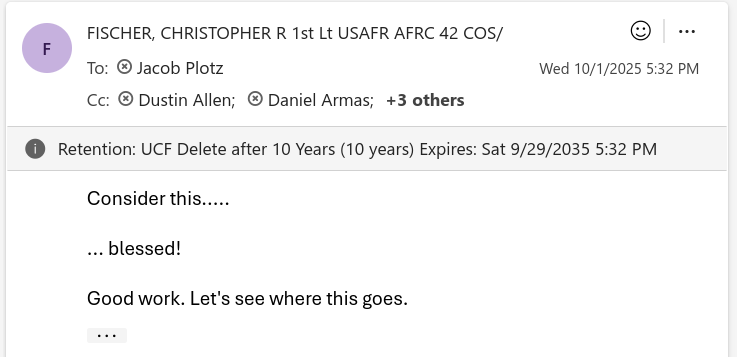
\includegraphics[width=\linewidth]{sponsor-email-screenshot.png}

\section{Team Contributions}
\subsection{Dustin Allen}
For my portion regarding the API implementation along with security needs I have been doing research on what possible API endpoints we will need. Aside from that I have also been looking into how to prevent people from using the AWS instance for malicious purposes. I have also been looking into how to get SSH working for our needs which I think I have a decent grasp currently on how to implement it. Based on what I’ve researched I think that I am ready to start work soon on coding the actual product.

\subsection{Rithik Dhakshnamoorthy}
I am currently doing research on dockerization and on how to deploy web apps on Docker. Right now, I have accomplished learning how to install Docker Engine, download containers, and run it for dockerization. I have even learned how I could delete containers if I wanted to. Interacting with Docker more lets me be able to know how I can use it for controlling containers.

\subsection{Daniel Armas}
For my part of the project, I have been learning how to utilize frontend technologies such as: REACT, Typescript, Javascript, and various CSS libraries. I have also practiced implementing these technologies in making a webpage with traits similar to what we are going to want for our project. I have also been scoping out websites and looking at how they design their home page and planing out what we would want our project to look like. After another week of practicing these skills and implementation, I would say that I would be ready to give it my all for this project.

\subsection{Jereme Saunders}
I am assigned the role of frontend developer, so most of my research has been related to developing my skills in that area, as I do not have much experience at all with it aside from some emergency attempts to fix issues on a project. I have been watching tutorials on YouTube and going through W3Schools tutorials on JavaScript and TypeScript.  I have also been going through code from a previous project for a web application where I did not do frontend development, but I understand the project well. This has been helpful because I can make the connection between what was done on the frontend side of things and compare it with what I see on the web page. To gain a broader understanding of the project, I have also conducted some research on Docker and containerization.

\section{Sprint Backlog}
\subsection{Sprint 1 (Weeks 1-3)}
\begin{itemize}
	\item Setup Database:
	      Select the database for the project. Create a schema or model of the data. Project scope is one user at a time, limited enough to allow for not putting much thought into the database. However, an approach that at least allows for the possibility of multiple users eliminates technical debt which may haunt future SD teams.
	\item Determine Essential Interactions:
	      Answer the question: what do our users want to do with Docker containers? The answer determines which API endpoints the backend must expose and which controls the UI team must anticipate.
	\item Create UI Mockups:
	      Create mockups/wireframes for the UI components of each page.
	\item Security Audit:
	      The entire team verifies the security practices used to set up the AWS instance. Each member documents potential issues with the setup.
	\item Select and Dockerize 7 Vulnerable Apps:
	      Select and containerize 7 appropriate vulnerable apps
\end{itemize}
\end{document}
